% begin module volumes-intro
\begin{frame}
\frametitle{Volumes}
\begin{center}
\begin{pspicture}(-3,-1.8)(3,3.3)
\renewcommand{\fcScreen}{[-1 -1 -1] 0}
\pscustom*[linecolor=cyan]{%
\fcPolyLineIIId{[-2 -2 0] [-2 2 0] [2 2 0] [2 -2 0] [-2 -2 0]}%
}%
\pscustom*[linecolor=white]{%
\fcCurveIIId{0}{360}{[2 t cos mul 2 t sin mul 0]}%
}%
%\fcAxesIIId{2}{2}{2}
\fcBoxIIId[linecolor=gray]{[2 2 2]}{[2 2 0]}{[2 -2 2]}{[-2 2 2]}%
\fcPlotIIIdXconst[linewidth=0.3pt, linecolor=\fcColorGraph]{iterationsX=15, iterationsY=15}{-2}{4 x x mul sub sqrt -1 mul}{2}{4 x x mul sub sqrt}{1 dict begin /rho x x mul y y mul  add sqrt def rho rho mul 2 rho  sub mul  0 max end}%
\fcPlotIIIdYconst[linewidth=0.3pt, linecolor=\fcColorGraph]{iterationsX=10, iterationsY=10}{4 y y mul sub sqrt -1 mul}{-2}{4 y y mul sub sqrt}{2}{1 dict begin /rho x x mul y y mul  add sqrt def rho rho mul 2 rho  sub mul  0 max end}%
\fcCurveIIId[linecolor=\fcColorGraph]{0}{360}{[2 t cos mul 2 t sin mul 0]}%
\end{pspicture}
%

Volumes of solids are found/defined via integration.%
\end{center}
\end{frame}

\begin{frame}
\begin{columns}[c]
\column{.35\textwidth}
\psset{xunit=2cm, yunit=2cm}
\begin{pspicture}(-0.3,-0.3)(2,1.2)%
\renewcommand{\fcScreen}{[-1 1.6 -1] 0}%
\fcBoundingBox{-0.3}{-0.3}{2}{1.2}%
\tiny%
\uncover<handout:0| 2>{%
\fcParallelogramIIId[linecolor=pink!70]{[0.3 0 0]}{[0.3 1 0]}{[0.3 0 1]}%
\fcParallelogramIIId[linecolor=cyan!70]{[0.3 0.35 0.35]}{[0.3 0.65 0.35]}{[0.3 0.35 0.65]}%
\fcParallelogramHalfVisibleIIId[linecolor=gray]{[0.3 0.35 0.65]}{[0.3 0.35 0.35]}{[0.3 0.65 0.65]}%
\fcPutIIId{[0.3 0.5 0.5]}{$A(x)$}%
\fcPutIIId[t]{[0.3 0 -0.1]}{$x$}%
}%
\uncover<handout:0| 3>{%
\fcParallelogramIIId[linecolor=pink!70]{[0.35 0 0]}{[0.35 1 0]}{[0.35 0 1]}%
\fcParallelogramIIId[linecolor=cyan!70]{[0.35 0.325 0.325]}{[0.35 0.675 0.325]}{[0.35 0.325 0.675]}%
\fcParallelogramHalfVisibleIIId[linecolor=gray!70]{[0.35 0.325 0.675]}{[0.35 0.325 0.325]}{[0.35 0.675 0.675]}%
\fcPutIIId{[0.35 0.5 0.5]}{$A(x)$}%
\fcPutIIId[t]{[0.35 0 -0.1]}{$x$}%
}%
\uncover<handout:0| 4>{%
\fcParallelogramIIId[linecolor=pink!70]{[0.4 0 0]}{[0.4 1 0]}{[0.4 0 1]}%
\fcParallelogramIIId[linecolor=cyan!70]{[0.4 0.3 0.3]}{[0.4 0.7 0.3]}{[0.4 0.3 0.7]}%
\fcParallelogramHalfVisibleIIId[linecolor=gray!70]{[0.4 0.3 0.7]}{[0.4 0.3 0.3]}{[0.4 0.7 0.7]}%
\fcPutIIId{[0.4 0.5 0.5]}{$A(x)$}%
\fcPutIIId[t]{[0.4 0 -0.1]}{$x$}%
}%
\uncover<handout:0| 5>{%
\fcParallelogramIIId[linecolor=pink!70]{[0.45 0 0]}{[0.45 1 0]}{[0.45 0 1]}%
\fcParallelogramIIId[linecolor=cyan!70]{[0.45 0.275 0.275]}{[0.45 0.725 0.275]}{[0.45 0.275 0.725]}%
\fcParallelogramHalfVisibleIIId[linecolor=gray!70]{[0.45 0.275 0.725]}{[0.45 0.275 0.275]}{[0.45 0.725 0.725]}%
\fcPutIIId{[0.45 0.5 0.5]}{$A(x)$}%
\fcPutIIId[t]{[0.45 0 -0.1]}{$x$}%
}%
\uncover<handout:1| 7->{%
\fcParallelogramIIId[linecolor=cyan!70]{[0.5 0.25 0.25]}{[0.5 0.75 0.25]}{[0.5 0.25 0.75]}%
\fcParallelogramHalfVisibleIIId[linecolor=gray!70]{[0.5 0.25 0.75]}{[0.5 0.25 0.25]}{[0.5 0.75 0.75]}%
}%
\uncover<6,7>{%
\fcParallelogramHalfVisibleIIId[linecolor=gray!70]{[0.4 0.3 0.7]}{[0.4 0.3 0.3]}{[0.4 0.7 0.7]}%
}
\uncover<7->{%
\fcPutIIId[t]{[0.5 0 -0.1]}{$x^*$}%
\fcLineIIId{[0.5 0 0]}{[0.5 0.05 0]}%
}%
\uncover<8->{%
\fcBoxIIIdFilled[linecolor=cyan!30]{[0.6 0.25 0.75]}{[0.4 0.25 0.75]}{[0.6 0.25 0.25]}{[0.6 0.75 0.75]}%
\fcParallelogramHalfVisibleIIId{[0.5 0.25 0.75]}{[0.5 0.25 0.25]}{[0.5 0.75 0.75]}%
\fcBoxIIId{[0.6 0.25 0.75]}{[0.4 0.25 0.75]}{[0.6 0.25 0.25]}{[0.6 0.75 0.75]}%
\fcLineIIId[arrows=<->]{[0.4 0.2 0.2]}{[0.6 0.2 0.2]}%
\fcPutIIId[t]{[0.5 0.16 0.16]}{$\Delta x$}%
}%
\fcLineIIId[arrows=->]{[0 0 0]}{[1.2 0 0]}%
\fcLineIIId[arrows=->]{[0 0 0]}{[0 1.2 0]}%
\fcLineIIId[arrows=->]{[0 0 0]}{[0 0 1.2]}%
\fcParallelogramHollowIIId{[1 0 0]}{[1 1 0]}{[1 0 1]}%
\fcLineIIId{[1 0 0]}{[0 0.5 0.5]}%
\fcLineIIId{[1 0 1]}{[0 0.5 0.5]}%
\fcLineIIId{[1 1 1]}{[0 0.5 0.5]}%
\fcLineIIId[linestyle=dashed]{[1 1 0]}{[0 0.5 0.5]}%
\uncover<6,7>{%
\fcParallelogramHalfVisibleIIId[linecolor=gray!70]{[0.6 0.2 0.8]}{[0.6 0.2 0.2]}{[0.6 0.8 0.8]}%
}%

\end{pspicture}

%\only<handout:1| -1>{%
%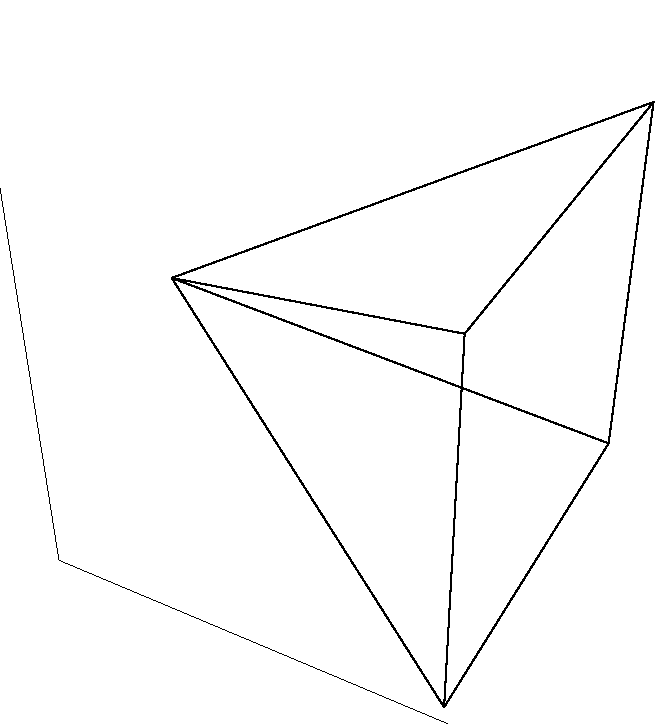
\includegraphics[height=4cm]{volumes/pictures/06-02-pyramida.pdf} %
%}%
%\only<handout:0| 2>{%
%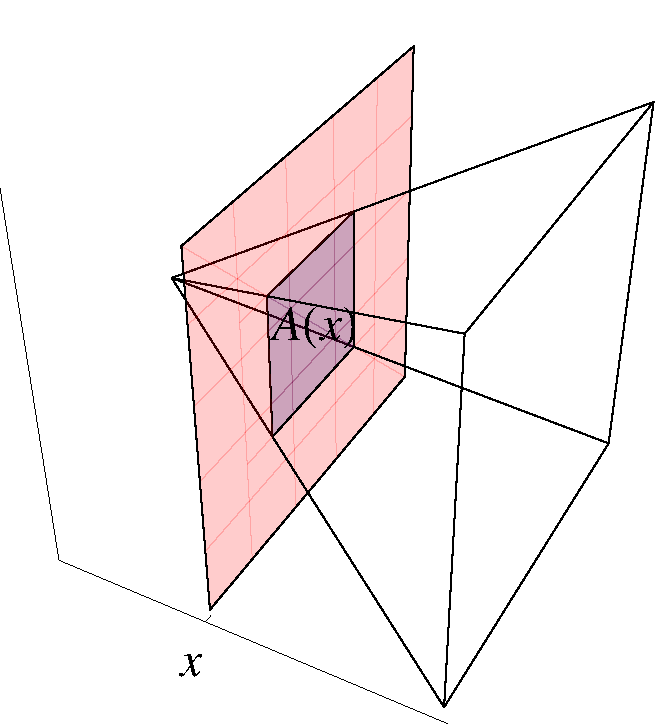
\includegraphics[height=4cm]{volumes/pictures/06-02-pyramidb.pdf}%
%}%
%\only<handout:0| 3>{%
%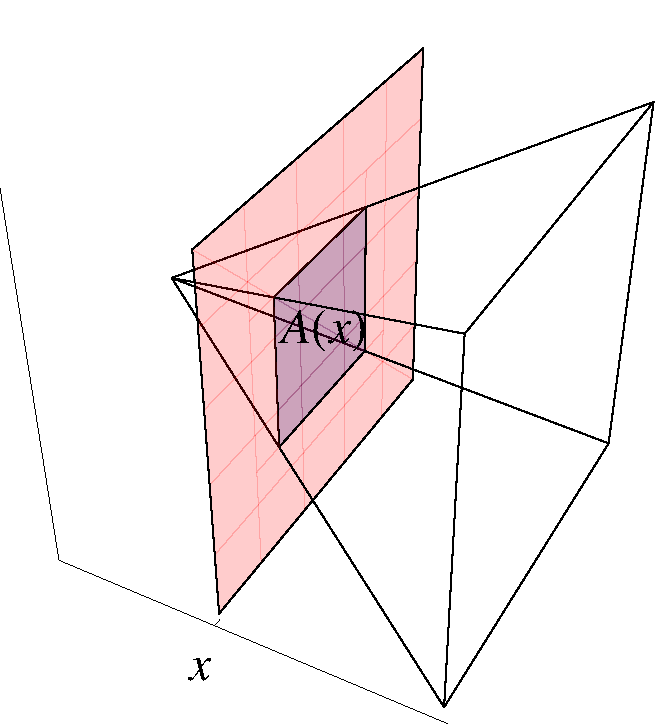
\includegraphics[height=4cm]{volumes/pictures/06-02-pyramidc.pdf}%
%}%
%\only<handout:0| 4>{%
%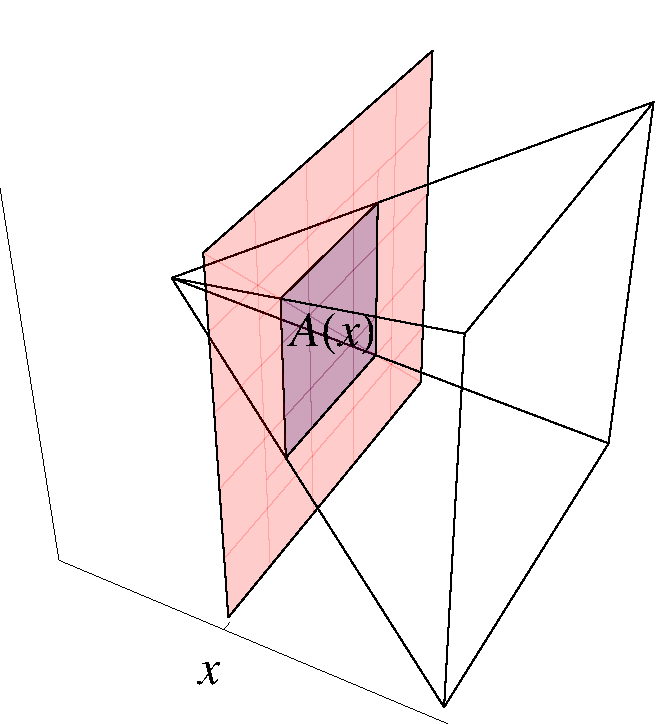
\includegraphics[height=4cm]{volumes/pictures/06-02-pyramidd.pdf}%
%}%
%\only<handout:2| 5>{%
%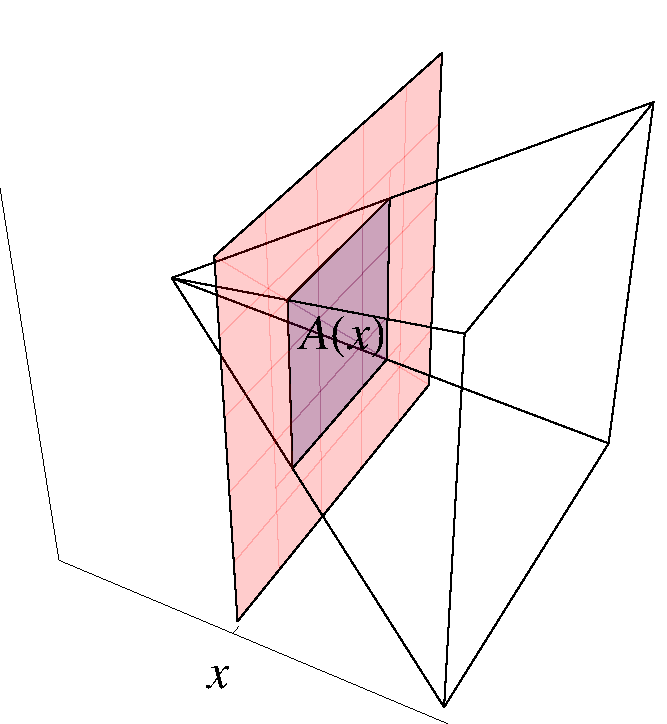
\includegraphics[height=4cm]{volumes/pictures/06-02-pyramide.pdf}%
%}%
%\only<handout:0| 6-7>{%
%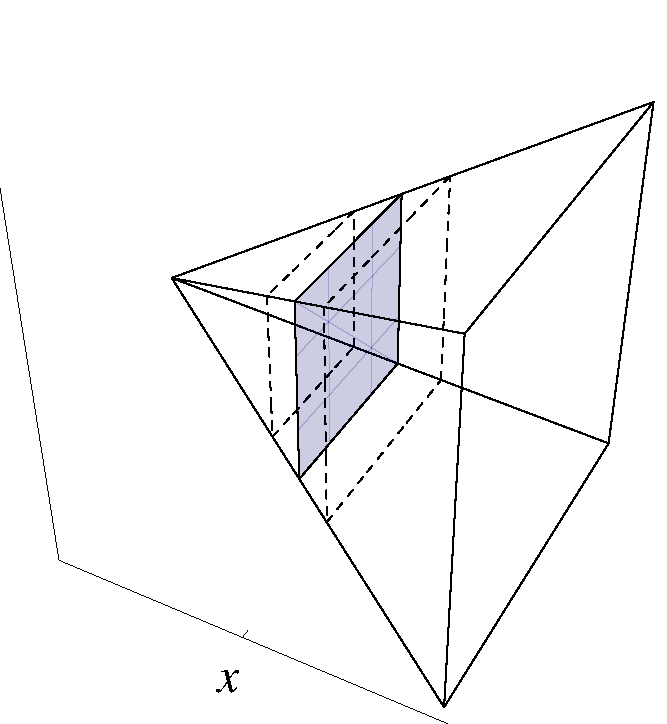
\includegraphics[height=4cm]{volumes/pictures/06-02-pyramidf.pdf}%
%}%
%\only<handout:3| 8->{%
%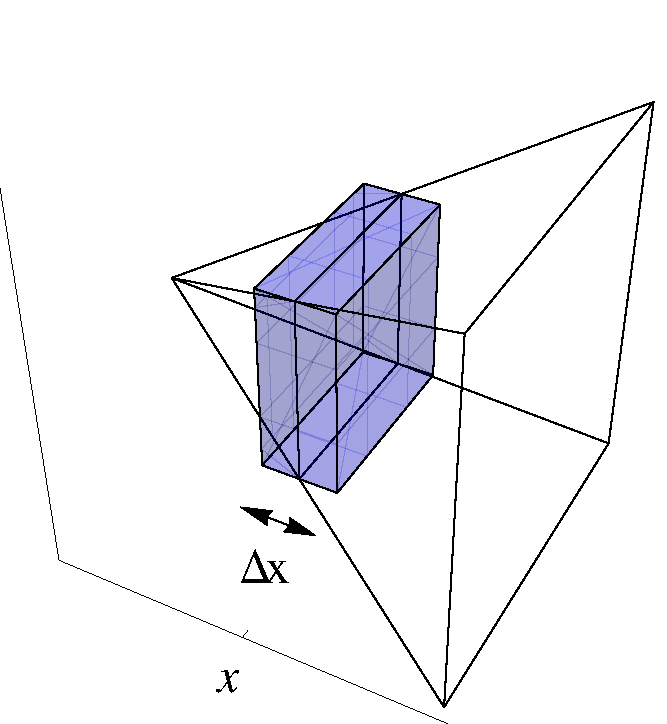
\includegraphics[height=4cm]{volumes/pictures/06-02-pyramidg.pdf}%
%}%

\uncover<handout:3| 9->{Approx. volume of slab:}
\abovedisplayskip=1pt
\belowdisplayskip=1pt
\[
\uncover<handout:3| 9->{A(x^*)\Delta x}%
\]
\uncover<handout:3| 10->{Approx. volume of $S$:}
\abovedisplayskip=1pt
\belowdisplayskip=1pt
\[
\uncover<handout:3| 10->{V \approx \sum_{i=1}^n A(x_i^*)\Delta x}%
\]
\uncover<handout:3| 11->{Exact volume of $S$:}
\abovedisplayskip=1pt
\belowdisplayskip=1pt
\[
\uncover<handout:3| 11->{V = \lim_{n\to\infty}\sum_{i=1}^n A(x_i^*)\Delta x}%
\]
\column{.65\textwidth}
\begin{itemize}
\item  How do we find the volume of a solid $S$?
\item<handout:2-| 2->  Let $P_x$ be the plane perpendicular to the $x$-axis and passing through the point $x$.
\item<handout:2-| 2->  The intersection of $P_x$ with $S$ is called a cross-section.
\item<handout:2-| 2->  Let $A(x)$ be the area of this cross-section.
\item<handout:3| 6->  Consider the part of $S$ between two planes $P_{x_1}$ and $P_{x_2}$.
\item<handout:3| 7->  Approximate this part of $S$:
\item<handout:3| 7->  Pick a sample point $x^*$ between $x_1$ and $x_2$.  Use a solid that has the same constant cross-sectional area $A(x^*)$ between $x_1$ and $x_2$.
\item<handout:3| 8->  Let $\Delta x$ be the distance from $x_1$ to $x_2$.
\end{itemize}
\end{columns}
\end{frame}
% end module volumes-intro
